\documentclass[conference]{IEEEtran}
\IEEEoverridecommandlockouts
% The preceding line is only needed to identify funding in the first footnote. If that is unneeded, please comment it out.
\usepackage{cite}
\usepackage{amsmath,amssymb,amsfonts}
\usepackage{algorithmic}
\usepackage{graphicx}
\usepackage{textcomp}
\usepackage{xcolor}
\usepackage{float}
\usepackage{kotex}
\def\BibTeX{{\rm B\kern-.05em{\sc i\kern-.025em b}\kern-.08em
    T\kern-.1667em\lower.7ex\hbox{E}\kern-.125emX}}
\begin{document}

\title{Farm Product Price Inform Service – NUGU FARM \\
\thanks{Identify applicable funding agency here. If none, delete this.}
}
\author{\IEEEauthorblockN{Kim Kwang Yeon}
\IEEEauthorblockA{\textit{Department of Information Systems} \\
\textit{College of Engineering}\\
Hanyang University\\
Seoul, Rep. of Korea \\
Email: kwang9705@gmail.com}
\\
\IEEEauthorblockN{Kim Jin Hyeok}
\IEEEauthorblockA{\textit{Department of Information Systems } \\
\textit{College of Engineering}\\
Hanyang University\\
Seoul, Rep. of Korea\\
Email: wlsgur948861@gmail.com
}
\\
\and
\IEEEauthorblockN{Kim Bong Kyun}
\IEEEauthorblockA{\textit{Department of Information Systems } \\
\textit{College of Engineering,}\\
Hanyang University\\
Seoul, Rep. of Korea\\
Email: qhdrnak@gmail.com }
\\
\IEEEauthorblockN{Choi Hyun Ji}
\IEEEauthorblockA{\textit{Department of Information Systems } \\
\textit{College of Engineering,}\\
Hanyang University\\
Seoul, Rep. of Korea\\
Email: tomz.seras@gmail.com}
}


\maketitle

\begin{abstract}
 
 
 For decades, government has been seeking solutions by setting price stability of agricultural products as its top priority. However, according to Ministry of Food and Drug Safety, crops with high consumer demand, such as potatoes and cabbage, are experiencing price fluctuations every two to three years due to various causes such as rising consumer prices and imports. In recent years, natural disasters such as floods and droughts have frequently occurred due to rapid changes in the climate environment, and as a result, the volatility of agricultural product prices is increasing more. Also, Fresh product delivery services have continued to increase due to the explosive increase in non-face-to-face delivery services since the COVID-19 incident and the prices fluctuate frequently and vary from company to company. At these reasons, NUGU Fresh was developed in consideration of the situation of agricultural products with such high price volatility. For those who often use early morning delivery, such as students living alone or those who don’t want to go and buy themselves, the prices of various companies’ early morning delivery crops are compared to the prices of marts and markets, and housewives and agricultural wholesalers can check the current market price and future price trends of agricultural products through NUGU speakers. In addition, sellers in traditional markets who are vulnerable to information can set standards for what prices to sell agricultural products.
\end{abstract}

\section{Introduction}
\subsection{Motivation}
    In recent years, prices of major agricultural products have soared along with rising consumer prices and natural disasters, causing inconvenience to consumers. For one example, typhoon damage occurs frequently from July to October when there is a holiday called Chuseok in Korea. In addition, when Chuseok approaches, most families buy holiday food ingredients, so consumer prices rise a lot. If a typhoon comes during this period, consumer prices can jump unimaginably. If this situation occurs, consumers may feel a great burden on prices. In anticipation of such impacts as natural disasters and increased demand, the government strives to stabilize prices by supplying more raw materials to the market to control prices. These supply and demand stabilization policies were promoted as a way to reduce the risk of price fluctuations, but detailed analysis is insufficient. Accurate analysis of how specific the price will change is still poor and decisions are made based on past experiences. If a high-accuracy agricultural product price prediction model could be created, it would be helpful to prepare in advance by predicting the section where these prices change severely.
    In addition, this prediction model is expected to help a lot at the personal level. Currently, many stories of housewives or wholesalers who are worried about agricultural prices are being introduced in the news. Housewives or wholesalers are often less familiar with electronic devices such as smartphones than younger people. In particular, elderly sellers who sell goods in traditional markets are bound to be more vulnerable to such price information. Currently, this agricultural price information can be found on a somewhat unfamiliar website called KAMIS. It only presents current and past prices here, but does not provide predictions of what future price information will be. Looking at this point, we wanted to create a service through artificial intelligence speakers that answers price information without complicated settings or access processes, and creating a homepage that can visualize and print such data to help these people. Housewives will be able to get a rough idea of when to buy agricultural products, and wholesalers will be able to set standards for what price to sell products in the coming future.
    Moreover, Fresh product delivery services have continued to increase due to the explosive increase in non-face-to-face delivery services since the COVID-19 incident. These services are very popular not only among young people, but also among middle-aged people between 50 and 60. According to a news article by ITWORLD, only 52\% of middle-aged people had experience using fresh products delivery in 2022 and nearly half of them used service frequently. Although the number of people using fresh product delivery services is increasing, there was no platform to compare the price of fresh product delivery sold by each company. In view of this inconvenience, we tried to provide the price information by NUGU speaker which is easy to access. As for the brands to compare prices, the representative brands of the three companies (Coupang Gomgom, Market Kurly KF365, SSG FRESH) and the average price of the mart and market provided by KAMIS were selected. Fresh products included in the top 30 heavily consumed foods selected by MFDS in Korea were chosen as the targets for price comparison. Through these services, At the same time, by predicting the prices of these fresh products, we intended to make it easier for consumers to choose by informing the trend of the prices of fresh products so that the timing of purchase could be determined easily



\subsection{Research on any related software}
\subsubsection{NUGU coin}

NUGU Coin service provides real-time coin market price information of the virtual asset exchange Bithumb. Coin information such as Bitcoin, Ethereum, and Ripple can be known, but market price errors may occur due to network and server failures.
\subsubsection{Ustockplus Chart Prediction Service}
The Ustockplus Chart Prediction Service analyzes past charts to predict the current most likely pattern and draws the predicted stock price on the stock chart. Ustockplus Chart Prediction Service analyzes the previous data statistically through its own prediction algorithm.
\subsubsection{Farm Morning}
Farm Morning notifies the national market price of agricultural products in real time. Farmers can immediately calculate how much they can earn from agricultural products harvested on the same day, so they can check the market price and sell agricultural products under the best conditions. It also provides weather information and cultivation information necessary for farming.\\

\begin{table}[!htbp]
\caption{ROLE ASSIGNMENTS}
\begin{tabular}{|c|c|p{2.5cm}|}
\hline
Roles& Name & Task descrption and etc\\
\hline 
user&Choi Hyun Ji & No matter how good the system is, it is meaningless if it is not easy to use from the user's point of view. He considers whether these services are easily accessible. If not, it suggests a way to develop service quality easily.\\
\hline
Customer& Kim Kwang yeon &Analyze the service from the buyer's point of view. Design services in consideration of appropriate costs and resources, and organize services to reach consumers attractively. \\
\hline
Software Developer & Kim Bong Kyun & Software developers design a full-scale software configuration. Write overall code without errors, and make the application do some tasks.\\
\hline
Development Manager& Kim Jin Hyeok & The development manager determines the overall software development process and appropriately distributes the schedule for each process. It also makes development easier by presenting tools that can be useful in the development process\\
\hline
\end{tabular}
\end{table}

\section{REQUIREMENTS}
\subsection{NUGU Speaker }\label{AA}
\subsubsection{Early Morning Delivery Price Comparing Service}
{a) Comparing Delivery Prices\\
When a user runs a NUGU farm and asks the price with the name of a particular crop, the AI speaker tells you the price when the crop is delivered in early morning. At this time, the price of crops is handled only for users who are located in Seoul, and when the user says other areas besides Seoul, the AI speaker says, "The area is not supported." The early morning delivery price standard tells you the cheapest of the three companies Coupang, E-Mart, and Market Kurly. For example, when a user asks, "Compare the price of cabbage in Seoul," the AI speaker compares the price of cabbage delivered at dawn by the three companies, and then speaks, "Coupang's cabbage price is the cheapest."}\\
\newline
{b) Comparing with current price
Compare the early morning delivery price of crops requested by users with the retail price at the current mart, so the users can choose whether buy crops by delivery or not. At this time, retail prices are also limited to those in Seoul.}

\subsubsection{Price notification service}
 a) Return historic market price:
You can know the past price of agricultural products through AI speakers. First, the user commands the speaker to “Start NUGU farm” or “Please turn on the price notification for agricultural products”. The speaker then gets the command, “NUGU farm has been executed”. To know the price, three characteristics are required: crop name, location and date, and if any of them are not met, the AI speaker does not return the price. For example, if a user says, “Tell me the price of cabbage in Seoul,” the AI speaker asks back, “Pleas tell me the date”, and if the user tells “a week ago,” then the speaker tells you the difference between the cabbage price and the cabbage price at the time of ignition a week ago in Seoul. Similarly, NUGU farm only deals with crops sold in Seoul, so when the user asks about other locations, AI Speaker will say, “NUGU farm notifies the prices of crops sold only in Seoul”, and continue the process later. The error message is repeated up to three times, and the AI speaker is terminated if the condition is not met after this.

b)  Return current market price
Similar to the past market price notification, if three factors are met and ordered, the current price is informed, and at the same time, the price change of the product is returned through the difference between the past market price and the current market price.

c) Forecasting future market prices
After satisfying the three elements, the command tells you the future predictors. However, future predictions can be made up to a week. When a user says, “Tell me the price of Seoul cabbage in a year”, it returns “NUGU farm can predict future prices up to a week”. When returning the future forecast, predicting price fluctuations through differences from the current price, “The price of radish on December 17 is expected to be 800 won per 100 grams. This is an increase of 80 won compared to the current forecast”.  As such, the direction of the market price of the relevant agricultural product is returned together.

\subsection{Website}
\subsubsection{Login/Logout}
After accessing the web page, the user can see the login page. If users have account, enter the email and password of the user account.  If the ID or password is wrong, use Find ID or Find Password located at the bottom of the input box. If user doesn't have an account, press the register button to go to the registration page. When users are done logging in, the showing data page is displayed. If login-ed user press the logout button, return to the login page immediately.
\subsubsection{Register}
Users enter their name, email, and password and click the Submit button to complete their registration.
\subsubsection{Show data}
The past/current/future price of the item received through the previous conversation can also be viewed through the web page. In addition, user can see a line graph showing the trend of price fluctuations from the past point in time to the present and one week later in a specific region. When the user requests the recommendation through conversation, he or she can receive the name of dish that can be made of the item, and also link to the recipe.
\subsubsection{Request data}
If user enters three characteristics of the crop name, sales area, and date in each input box, user can receive information like the previous 3) Show data.
\subsection{Additional Functions}
\subsubsection{Setting speed of speech}
Adding an in-sentence speech option tag allows users to communicate smoothly with NUGU. Since NUGU Farm is designed for housewives or information-vulnerable groups rather than young people in their 20s and 30s, it sets the utterance speed set to 100\% default to 85\% of NUGU's lowest recommended speed. In addition, before informing the price it creates an environment where users can focus more on the price by setting small period of term before price information through the strong attribute.

\section{DEVELOPMENT ENVIRONMENT}
\subsection{Choice of Software Development Platform}
\subsubsection{Programming Language}
\begin{figure}[!htbp]
\centering
    
\includegraphics[width =4.5cm]{python}
    \hfil
\caption{python}
\label{python}
\end{figure}

{a)	Python\\
-	Python is high-level programming language which is interpreted and object-oriented. Easy to learn and use Python, which is useful for readability, reduces program maintenance costs. Python supports a variety of modules and packages and pursues program modularization. In particular, it is widely used in data-related fields, supporting modules related to data-specific such as Pandas and Numpy.}

\subsubsection{Development Environment}

\begin{figure}[!htbp]
\centering
    
\includegraphics[width =4.5cm]{django}
    \hfil
\caption{Django}
\end{figure}
a)	Django\\

-	Django is an advanced Python web framework which pursues practical design and efficient development. Many of the features already created, such as Django Admin, Form, and Serializer, deal with much of the inconvenience of web development, so you don't have to recreate the new features from scratch, just use them. You can also save money as a free open source.

\begin{figure}[!htbp]
\centering
    
\includegraphics[width =4.5cm]{keras}
    \hfil
\caption{Keras}
\end{figure}
b)	Keras
-	Keras is a deep learning API designed to be human-friendly rather than machine-friendly. Keras was born with great effort to reduce cognitive load. Provides a simple, consistent API, and provides clear, actionable error messages. It also includes a wide range of user manuals, making it easier for users to use.
\newpage
\begin{figure}[!htbp]
\centering
    
\includegraphics[width =4.5cm]{airflow.eps}
    \hfil
\caption{Airflow}
\end{figure}

c)	Airflow
-	Apache Airflow is an open-source workflow management platform created for data engineering pipelines. This allows you to manage and monitor complex workflows. It uses directed acyclic graphs (DAGs) to manage workflow coordination. Then, it manages scheduling and execution that can be executed by a defined schedule.

\begin{figure}[!htbp]
\centering
    
\includegraphics[width =4.5cm]{ncp.eps}
    \hfil
\caption{Naver Cloud Platform}
\end{figure}

d)	Naver Cloud Platform
-	Naver Cloud Platform is an enterprise cloud service provided by Naver Cloud. From basic IaaS such as servers and storage to PaaS, and SaaS, a business collaboration platform such as WORKPLACE. Naver affiliates such as Line, Naver Webtoon, and V-Live are using Naver Cloud Platform, and many large companies have also introduced Naver Cloud Platform services.

\begin{figure}[!htbp]
\centering
    
\includegraphics[width =4.5cm]{AWS.eps}
    \hfil
\caption{AWS}
\end{figure}
e)	Amazon Web Services
-	Amazon Web Services (AWS) platform provides more than 200 fully featured services from data centers located all over the world, and is the world's most comprehensive cloud platform. It provides scalable and cost-effective cloud solutions such as computer power, database storage, content delivery, etc. 

\begin{figure}[!htbp]
\centering
    
\includegraphics[width =4.5cm]{github.eps}
    \hfil
\caption{GitHub}
\end{figure}

f)	GitHub
-	GitHub is a web-based version-control and collaboration platform for software developers. Git is used to store the source code for a project and track the complete history of all changes to that code. It allows developers to collaborate on a project more effectively by providing tools for managing possibly conflicting changes from multiple developers.

\begin{figure}[!htbp]
\centering
    
\includegraphics[width =4.5cm]{nuguplaybuilder.eps}
    \hfil
\caption{Nugu Play Builder}
\end{figure}

g)	NUGU Play Builder
-	NUGU play is a unit of service in response to a user's request through the NUGU platform, and you can create Play in the Play Builder. It helps companies or individuals with good content to provide their services to NUGU users through Play. The User Utterance Model, which understands the user's speech, and then identifies the user's Intent and combines actions that perform functions based on it to create a complete play.

\begin{figure}[!htbp]
\centering
    
\includegraphics[width =4.5cm]{twilio.eps}
    \hfil
\caption{Twillo}
\end{figure}
h)	Twilio
-	Twilio is a US cloud communication platform as a service (CPaaS) that allows software developers to semi-automatically build business communication processes. Twilio helps its clients focus on their current goals, like communication with partners, customers, and employees instead of spending a huge amount of time negotiating with mobile operators to solve communication problems.\\


\subsection{Cost Estimation}

\begin{table}[h]
\begin{tabular}{|c|c|c|}
\hline
Service               & Region             & Cost(hourly)                       \\
\hline
Amazon EC2 p3.2xlarge & North East (Seoul) & 3.06 USD                           \\
\hline
Naver Ncloud Compact  & Korea              & 48 WON                             \\
\hline
Amazon RDS            & North East (Seoul) & Cost is required after 750   hours\\
\hline
\end{tabular}
\end{table}

\subsection{Development Environment Description}
\begin{table}[h]
\begin{tabular}{|c|c|p{2.5cm}|}
\hline
Name   & Version       & Description                  \\ \hline
Windows            & 10 Home & graphical operating system   developed and published by Microsoft.  \\ \hline
Ubuntu & 16.04 (64bit) & Linux-based operating system \\ \hline
Visual Studio code & 1.72    & Source-code editor made by   Microsoft with the Electron Framework, \\ \hline
\end{tabular}
\end{table}


\subsection{Software in use}
There are websites that compare the prices of various products such as Danawa and Enuri. However, these websites did not directly compare the prices of Coupang, Market Kurly, and SSG, the most popular fresh product delivery platforms. It also did not show what trend prices will change in the future. By comparing these fresh product deliveries to the average price sold at the mart, our NUGU farm make consumers to choose the right choice, and by asking the speaker questions without having to bother comparing directly from the mobile phone through the website.\\

\subsection{Task Distribution}

\begin{table}[h]
\begin{tabular}{|l|l|}
\hline
Name           & Task description   \\ \hline
Kim Kwang Yeon & Play Builder,   AI \\ \hline
Kim Jin Hyeok  & Backend, AI        \\ \hline
Kim Bong Kyun  & Backend, AI        \\ \hline
Choi Hyun Ji   & Play Builder,   AI \\ \hline
\end{tabular}
\end{table}
Basically, each group of two is in charge of one part each.  



\section{Specification}
\subsection{NUGU Speaker}
\subsubsection{Early Morning Delivery Price Comparing Service\\}
\begin{figure}[b]
\centering
    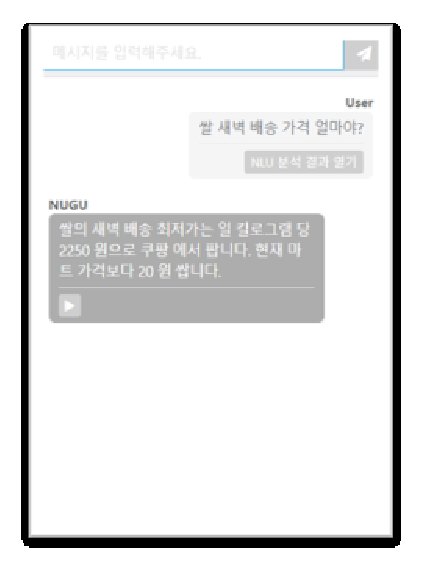
\includegraphics[width =4.5cm]{1-1.eps}
    \hfil
\caption{Early Morning Delivery Price Service}
\end{figure}
This service is a price notification service for agricultural products targeting the Seoul area. If a user requests a price outside of Seoul, such as “대전 배추 가격 알려줘” then speaker returns "지역은 서울만 가능합니다. 서울 가격을 알려드릴까요?" This service compares the prices of early morning delivery services of the three companies "Coupang," "Market Curly" and "SSG.COM" and returns the prices of the cheapest one to users. In addition, it can be compared with the price of the local market in conjunction with the agricultural product price notification service. When the user says to the speaker, " NUGU FARM 실행해줘” The speaker will run service with “NUGU FARM 실행합니다. 원하는 작물을 말해주세요” In addition, services can be called up as "NUGU FARM 실행", "NUGU FARM", or " 농산물 가격 정보 실행.” After the procedure is complete, the speaker returns “해당 상품의 과거 가격 혹은 미래 가격을 알려드릴까요?”를 Users can use the service through "그래", "어", etc., or terminate NUGU FARM through "종료." This function is a price notification service for agricultural products targeting the Seoul area. If a user requests a price outside of Seoul, such as "Tell me the price of Daejeon cabbage," it returns "The area is not supported." The function compares the prices of early morning delivery services of the three companies "쿠팡" "마켓컬리" and "쓱닷컴" and returns the prices of the cheapest one to users. At the end it compares the price of the local market





a) Return historic market price:
When the user asks to start NUGU farm “누구 팜 시작”, the AI speaker will ask “안녕하세요, 누구 팜 입니다. 무엇을 도와드릴까요?” The user ask price of crops he wants. At this time, AI Speaker requires three characteristics: crop name, date, and location. The types of crops include rice, cabbage, apples, onions, radishes, potatoes, cucumbers, and tomatoes, but when you ask about other crops, AI speaker says “해당 농작물은 지원하지 않습니다.” Also, the location is only for Seoul, but if the user ask about other areas, AI Speaker answers “지역은 서울만 가능합니다. 서울 가격을 알려드릴까요?.” Likewise, if the user doesn’t include location, AI Speaker says “날짜를 알려주세요.” These error messages are repeated up to three times, and the AI speaker is terminated “누구 팜을 종료합니다,” if the conditions are not met after this. If the user ask “어제 서울 쌀 가격 알려줘,” then AI speaker answers requested crops’ price, and difference between price of yesterday and the point of utterance at that time “어제 서울의 쌀 가격은 1kg 당 OOO원 입니다. 현재 가격과 OOO원 차이 납니다.”

\subsubsection{Price notification service\\}
\begin{figure}[h]
\centering
    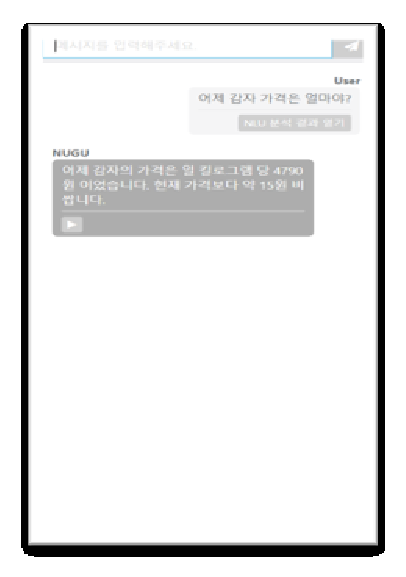
\includegraphics[width =4.5cm]{1-2.eps}
    \hfil
\caption{Return historic market price(date O\\}
\end{figure}

\begin{figure}[h]
\centering
    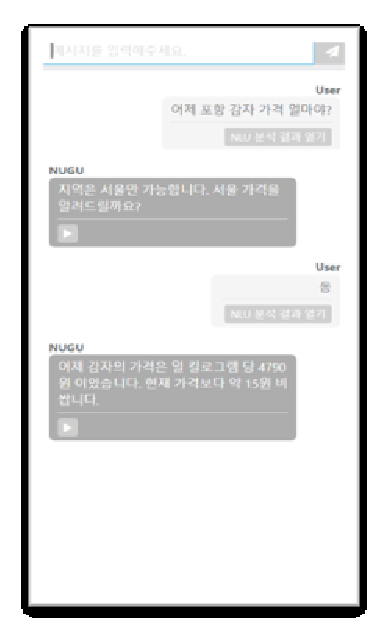
\includegraphics[width =4.5cm]{1-3.eps}
    \hfil
\caption{Return historic market price(No location)}
\end{figure}
\newpage

b)Forecasting future market prices
After satisfying the three characteristics, the AI speaker tells you the future predictors. If the user asks “내일 서울 배추 가격 알려줘”, AI speaker answers “내일 서울 배추의 가격은 1 k당 OOO원으로 예상됩니다. 현재 가격과는 OOO원 차이 납니다.” However, NUGU farm can only possible to predict up to a week, so when the user asks price after a week, AI speaker says “해당 날짜는 지원하지 않습니다.” As such, the direction of the market price of the relevant agricultural product is returned together.

\begin{figure}[h]
\centering
    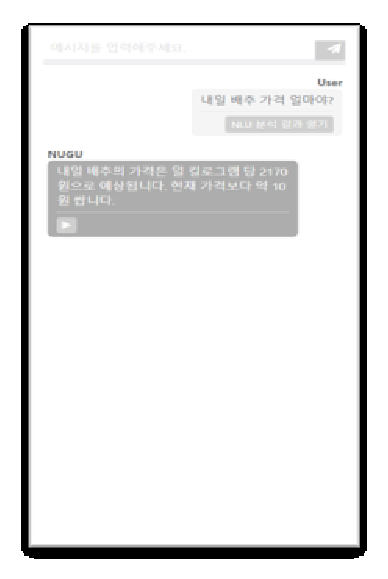
\includegraphics[width =4.5cm]{1-4.eps}
    \hfil
\caption{ Forecasting future prices}
\end{figure}

\begin{figure}[h]
\centering
    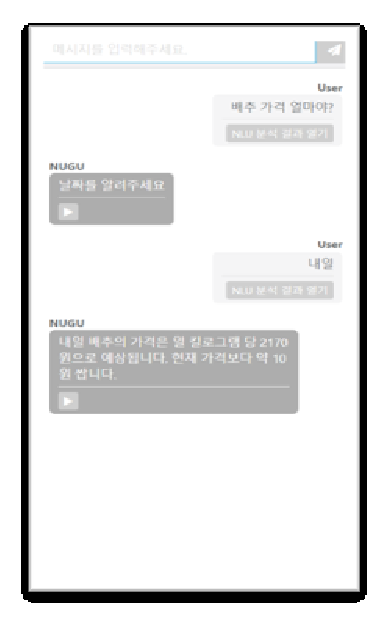
\includegraphics[width =4.5cm]{1-5.eps}
    \hfil
\caption{ Forecasting future prices(date) }
\end{figure}
\newpage
\subsubsection{Additional Function}
1) Setting speed of speech
When you convert a NUGU speaker's response prompt to voice, you can make it read the way you want it. NUGU speaker is made for the vulnerable, primarily the elderly. The ignition speed was defaulted to the lowest recommended speed of 85\%. You can also adjust the pitch. The pitch is 100\% basic, and the parts that need to be emphasized such as price and product name are set at 105\%. You can adjust the length of silence after reading the sentences, and the main information such as price and product name has increased the existing 300ms to 500ms. By highlighting the key words, the information can be communicated even if the user does not understand the whole context.

\subsection{Message sending service}
At the end of conversation between NUGU AI speaker and user, AI speaker asks ‘Do you want me to text you the information so far?’ If user answers ‘yes’ and if the user's phone number is already registered, it immediately sends a message containing the price information so far, or if not registered, AI speaker asks the user for the phone number and registers it before sending the message. The example message will be like Fig. 15 below. When user answers ‘no’ for the messaging suggestion, AI speaker answers like “NUGU Fresh를 종료합니다” and turns off NUGU Fresh.

\begin{figure}[h]
\centering
    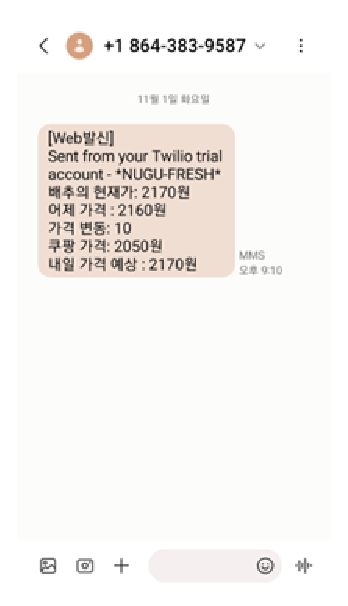
\includegraphics[width =4.5cm]{1-6.eps}
    \hfil
\caption{Message sending service}
\end{figure}
\newpage

\subsection{Equations}
Number equations consecutively. To make your 
equations more compact, you may use the solidus (~/~), the exp function, or 
appropriate exponents. Italicize Roman symbols for quantities and variables, 
but not Greek symbols. Use a long dash rather than a hyphen for a minus 
sign. Punctuate equations with commas or periods when they are part of a 
sentence, as in:
\begin{equation}
a+b=\gamma\label{eq}
\end{equation}

Be sure that the 
symbols in your equation have been defined before or immediately following 
the equation. Use ``\eqref{eq}'', not ``Eq.~\eqref{eq}'' or ``equation \eqref{eq}'', except at 
the beginning of a sentence: ``Equation \eqref{eq} is . . .''

\subsection{\LaTeX-Specific Advice}

Please use ``soft'' (e.g., \verb|\eqref{Eq}|) cross references instead
of ``hard'' references (e.g., \verb|(1)|). That will make it possible
to combine sections, add equations, or change the order of figures or
citations without having to go through the file line by line.

Please don't use the \verb|{eqnarray}| equation environment. Use
\verb|{align}| or \verb|{IEEEeqnarray}| instead. The \verb|{eqnarray}|
environment leaves unsightly spaces around relation symbols.

Please note that the \verb|{subequations}| environment in {\LaTeX}
will increment the main equation counter even when there are no
equation numbers displayed. If you forget that, you might write an
article in which the equation numbers skip from (17) to (20), causing
the copy editors to wonder if you've discovered a new method of
counting.

{\BibTeX} does not work by magic. It doesn't get the bibliographic
data from thin air but from .bib files. If you use {\BibTeX} to produce a
bibliography you must send the .bib files. 

{\LaTeX} can't read your mind. If you assign the same label to a
subsubsection and a table, you might find that Table I has been cross
referenced as Table IV-B3. 

{\LaTeX} does not have precognitive abilities. If you put a
\verb|\label| command before the command that updates the counter it's
supposed to be using, the label will pick up the last counter to be
cross referenced instead. In particular, a \verb|\label| command
should not go before the caption of a figure or a table.

Do not use \verb|\nonumber| inside the \verb|{array}| environment. It
will not stop equation numbers inside \verb|{array}| (there won't be
any anyway) and it might stop a wanted equation number in the
surrounding equation.

\subsection{Some Common Mistakes}\label{SCM}
\begin{itemize}
\item The word ``data'' is plural, not singular.
\item The subscript for the permeability of vacuum $\mu_{0}$, and other common scientific constants, is zero with subscript formatting, not a lowercase letter ``o''.
\item In American English, commas, semicolons, periods, question and exclamation marks are located within quotation marks only when a complete thought or name is cited, such as a title or full quotation. When quotation marks are used, instead of a bold or italic typeface, to highlight a word or phrase, punctuation should appear outside of the quotation marks. A parenthetical phrase or statement at the end of a sentence is punctuated outside of the closing parenthesis (like this). (A parenthetical sentence is punctuated within the parentheses.)
\item A graph within a graph is an ``inset'', not an ``insert''. The word alternatively is preferred to the word ``alternately'' (unless you really mean something that alternates).
\item Do not use the word ``essentially'' to mean ``approximately'' or ``effectively''.
\item In your paper title, if the words ``that uses'' can accurately replace the word ``using'', capitalize the ``u''; if not, keep using lower-cased.
\item Be aware of the different meanings of the homophones ``affect'' and ``effect'', ``complement'' and ``compliment'', ``discreet'' and ``discrete'', ``principal'' and ``principle''.
\item Do not confuse ``imply'' and ``infer''.
\item The prefix ``non'' is not a word; it should be joined to the word it modifies, usually without a hyphen.
\item There is no period after the ``et'' in the Latin abbreviation ``et al.''.
\item The abbreviation ``i.e.'' means ``that is'', and the abbreviation ``e.g.'' means ``for example''.
\end{itemize}
An excellent style manual for science writers is \cite{b7}.

\subsection{Authors and Affiliations}
\textbf{The class file is designed for, but not limited to, six authors.} A 
minimum of one author is required for all conference articles. Author names 
should be listed starting from left to right and then moving down to the 
next line. This is the author sequence that will be used in future citations 
and by indexing services. Names should not be listed in columns nor group by 
affiliation. Please keep your affiliations as succinct as possible (for 
example, do not differentiate among departments of the same organization).

\subsection{Identify the Headings}
Headings, or heads, are organizational devices that guide the reader through 
your paper. There are two types: component heads and text heads.

Component heads identify the different components of your paper and are not 
topically subordinate to each other. Examples include Acknowledgments and 
References and, for these, the correct style to use is ``Heading 5''. Use 
``figure caption'' for your Figure captions, and ``table head'' for your 
table title. Run-in heads, such as ``Abstract'', will require you to apply a 
style (in this case, italic) in addition to the style provided by the drop 
down menu to differentiate the head from the text.

Text heads organize the topics on a relational, hierarchical basis. For 
example, the paper title is the primary text head because all subsequent 
material relates and elaborates on this one topic. If there are two or more 
sub-topics, the next level head (uppercase Roman numerals) should be used 
and, conversely, if there are not at least two sub-topics, then no subheads 
should be introduced.

\subsection{Figures and Tables}
\paragraph{Positioning Figures and Tables} Place figures and tables at the top and 
bottom of columns. Avoid placing them in the middle of columns. Large 
figures and tables may span across both columns. Figure captions should be 
below the figures; table heads should appear above the tables. Insert 
figures and tables after they are cited in the text. Use the abbreviation 
``Fig.~\ref{fig}'', even at the beginning of a sentence.

\begin{figure}[htbp]
\centerline{\includegraphics{fig1.png}}
\caption{Example of a figure caption.}
\label{fig}
\end{figure}

Figure Labels: Use 8 point Times New Roman for Figure labels. Use words 
rather than symbols or abbreviations when writing Figure axis labels to 
avoid confusing the reader. As an example, write the quantity 
``Magnetization'', or ``Magnetization, M'', not just ``M''. If including 
units in the label, present them within parentheses. Do not label axes only 
with units. In the example, write ``Magnetization (A/m)'' or ``Magnetization 
\{A[m(1)]\}'', not just ``A/m''. Do not label axes with a ratio of 
quantities and units. For example, write ``Temperature (K)'', not 
``Temperature/K''.

\section*{Acknowledgment}

The preferred spelling of the word ``acknowledgment'' in America is without 
an ``e'' after the ``g''. Avoid the stilted expression ``one of us (R. B. 
G.) thanks $\ldots$''. Instead, try ``R. B. G. thanks$\ldots$''. Put sponsor 
acknowledgments in the unnumbered footnote on the first page.

\section*{References}

Please number citations consecutively within brackets \cite{b1}. The 
sentence punctuation follows the bracket \cite{b2}. Refer simply to the reference 
number, as in \cite{b3}---do not use ``Ref. \cite{b3}'' or ``reference \cite{b3}'' except at 
the beginning of a sentence: ``Reference \cite{b3} was the first $\ldots$''

Number footnotes separately in superscripts. Place the actual footnote at 
the bottom of the column in which it was cited. Do not put footnotes in the 
abstract or reference list. Use letters for table footnotes.

Unless there are six authors or more give all authors' names; do not use 
``et al.''. Papers that have not been published, even if they have been 
submitted for publication, should be cited as ``unpublished'' \cite{b4}. Papers 
that have been accepted for publication should be cited as ``in press'' \cite{b5}. 
Capitalize only the first word in a paper title, except for proper nouns and 
element symbols.

For papers published in translation journals, please give the English 
citation first, followed by the original foreign-language citation \cite{b6}.

\begin{thebibliography}{00}
\bibitem{b1} G. Eason, B. Noble, and I. N. Sneddon, ``On certain integrals of Lipschitz-Hankel type involving products of Bessel functions,'' Phil. Trans. Roy. Soc. London, vol. A247, pp. 529--551, April 1955.
\bibitem{b2} J. Clerk Maxwell, A Treatise on Electricity and Magnetism, 3rd ed., vol. 2. Oxford: Clarendon, 1892, pp.68--73.
\bibitem{b3} I. S. Jacobs and C. P. Bean, ``Fine particles, thin films and exchange anisotropy,'' in Magnetism, vol. III, G. T. Rado and H. Suhl, Eds. New York: Academic, 1963, pp. 271--350.
\bibitem{b4} K. Elissa, ``Title of paper if known,'' unpublished.
\bibitem{b5} R. Nicole, ``Title of paper with only first word capitalized,'' J. Name Stand. Abbrev., in press.
\bibitem{b6} Y. Yorozu, M. Hirano, K. Oka, and Y. Tagawa, ``Electron spectroscopy studies on magneto-optical media and plastic substrate interface,'' IEEE Transl. J. Magn. Japan, vol. 2, pp. 740--741, August 1987 [Digests 9th Annual Conf. Magnetics Japan, p. 301, 1982].
\bibitem{b7} M. Young, The Technical Writer's Handbook. Mill Valley, CA: University Science, 1989.
\end{thebibliography}
\vspace{12pt}
\color{red}
IEEE conference templates contain guidance text for composing and formatting conference papers. Please ensure that all template text is removed from your conference paper prior to submission to the conference. Failure to remove the template text from your paper may result in your paper not being published.

\end{document}%%
